\section*{Завдання 1}
Побудувати граф досяжних розміток мережі Петрі.

\usetikzlibrary{arrows.meta}

\begin{center}
    \begin{tikzpicture}
    [node distance=1.3cm,on grid,>=stealth',bend angle=30,auto,
    every place/.style= {minimum size=6mm,thick,draw=blue!75,fill=blue!20},
    every transition/.style={thick,draw=black!75,fill=black!20},
    red place/.style= {place,draw=red!75,fill=red!20}]

    \node [place] at (-3, 2) (A) {1};
    \node [place] at (-3, 0) (B) {2};
    \node [place] at (3, 2) (C) {3};
    \node [place] at (3, 0) (D) {4};
    \node [place,tokens=1] at (0, -2) (E) {\hspace{0.3cm} 5};

    \node [transition] at (-6, 1) (t1) {A}
    edge [pre, bend right] (E)
    edge [post] (A)
    edge [post] (B);

    \node [transition] at (0, 2) (t2) {B}
    edge [pre] (A)
    edge [post] (C);

    \node [transition] at (0, 0) (t3) {C}
    edge [pre] (B)
    edge [post] (D);

    \node [transition] at (6, 1) (t4) {D}
    edge [pre] (C)
    edge [pre] (D)
    edge [post, bend left] (E)
    edge [post, bend left=10] (A);

    \end{tikzpicture}
\end{center}

\begin{center}
    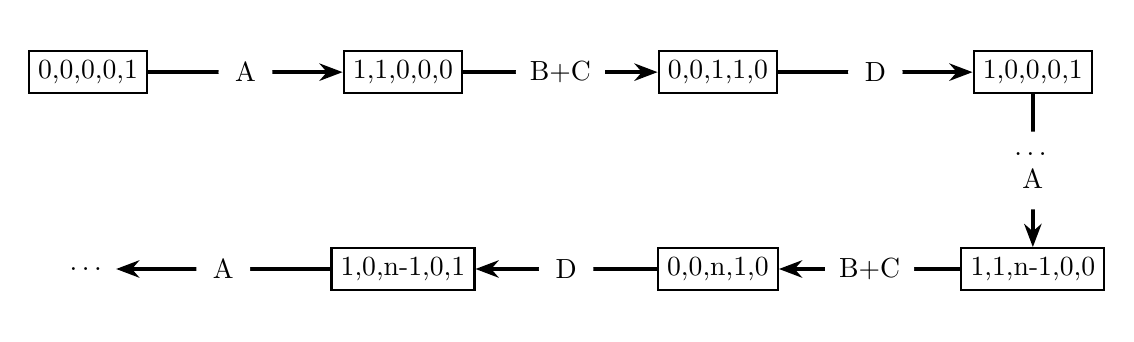
\begin{tikzpicture}
        \begin{scope}[every node/.style={rectangle,thick,draw}]
            \node (A) at (-12,0) {0,0,0,0,1};
            \node (B) at (-8,0) {1,1,0,0,0};
            \node (C) at (-4,0) {0,0,1,1,0};
            \node (D) at (0, 0) {1,0,0,0,1};
            \node (E) at (0, -2.5) {1,1,n-1,0,0};
            \node (F) at (-4,-2.5) {0,0,n,1,0};
            \node (G) at (-8,-2.5) {1,0,n-1,0,1};
        \end{scope}

        \node (H) at (-12, -2.5) {\dots};

        \begin{scope}[>={Stealth[black]},
            every node/.style={fill=white,circle},
            every edge/.style={very thick, draw}]
            \path [->] (A) edge node{A} (B);
            \path [->] (B) edge node{B+C} (C);
            \path [->] (C) edge node{D} (D);
            \path [->] (D) edge node[align=center]{\dots \\ A} (E);
            \path [->] (E) edge node{B+C} (F);
            \path [->] (F) edge node{D} (G);
            \path [->] (G) edge node{A} (H);
        \end{scope}
    \end{tikzpicture}
\end{center}

Де $n$ - номер "ітерації" у циклі, який є у графі, що відповідає мережі
Петрі(кількість разів, коли перехід A був виконаним).

Як ми можемо бачити мережі Петрі не відповідає мова,
яка допускає скінченне слово(у графі досяжних розміток
нескінченність вершин та немає термінальних вершин).